\documentclass[11pt,a4paper]{article}

\usepackage[T1]{fontenc}
\usepackage[utf8]{inputenc}
\usepackage[french]{babel}
\usepackage{lmodern}
\usepackage{microtype}
\usepackage{geometry}
\usepackage{graphicx}
\usepackage{booktabs}
\usepackage{float}
\usepackage{caption}
\usepackage{hyperref}
\usepackage{xcolor}
\usepackage{listings}
\usepackage{fancyhdr}
\usepackage{enumitem}
\usepackage{array}
\usepackage{longtable}

\geometry{margin=2.5cm}
\hypersetup{colorlinks=true, linkcolor=blue!60!black, urlcolor=blue!70!black, citecolor=blue!60!black}
\pagestyle{fancy}
\fancyhf{}
\fancyhead[L]{\small Rapport projet RAG --- NLP M1}
\fancyhead[R]{\small Mohamed Salem Ebnou Echvagha Oubeid}
\fancyfoot[C]{\thepage}

% --- Logo: change this path in Overleaf if needed ---
\newcommand{\UniversityLogoPath}{figures/university_logo.png}

\definecolor{codebg}{RGB}{245,245,245}
\definecolor{codeframe}{RGB}{200,200,200}
\lstdefinestyle{python}{
  language=Python,
  basicstyle=\ttfamily\small,
  backgroundcolor=\color{codebg},
  frame=single,
  rulecolor=\color{codeframe},
  breaklines=true,
  columns=fullflexible,
  keepspaces=true,
  showstringspaces=false,
  keywordstyle=\color{blue!70!black},
  commentstyle=\color{gray},
  stringstyle=\color{teal!60!black},
  numbers=left,
  numberstyle=\tiny\color{gray},
  numbersep=8pt,
  tabsize=4,
}

\title{%
  \vspace{-1cm}
  {\Large Module NLP --- Master 1, Semestre 2, 2025--2026}\\[0.8cm]
  {\LARGE Conception d'un syst\`eme RAG}\\[0.4cm]
  {\large Assistant question-r\'eponse sur les concepts de NLP / Machine Learning}
}
\author{Mohamed Salem Ebnou Echvagha Oubeid --- C34613}
\date{Rapport de projet --- Retrieval-Augmented Generation\\[0.2cm]
      D\'ep\^ot Git : \url{https://github.com/Muhammed-OTP/rag-nlp-m1}}

\begin{document}

% --- Page de garde ---
\begin{titlepage}
  \centering
  \includegraphics[width=3.2cm]{\UniversityLogoPath}\\[1.2cm]
  {\large Module NLP --- Master 1, Semestre 2, 2025--2026}\\[1.5cm]
  {\LARGE\bfseries Conception d'un syst\`eme RAG}\\[0.5cm]
  {\large Assistant question-r\'eponse sur les concepts de NLP / Machine Learning}\\[2cm]
  {\large\bfseries Auteur :}\\[0.2cm]
  Mohamed Salem Ebnou Echvagha Oubeid --- C34613\\[1.5cm]
  {\large Domaine choisi :}\\[0.2cm]
  Concepts fondamentaux du traitement automatique du langage naturel (NLP) et du machine learning,
  \`a partir d'un corpus d'articles Wikipedia en anglais.\\[1.5cm]
  {\large D\'ep\^ot GitHub :}\\[0.2cm]
  \url{https://github.com/Muhammed-OTP/rag-nlp-m1}\\[1.5cm]
  \today
\end{titlepage}

\tableofcontents
\newpage

\section{Introduction}

Ce projet a \'et\'e r\'ealis\'e dans le cadre du module NLP du Master~1. Il consiste \`a concevoir,
impl\'ementer et \'evaluer un syst\`eme de \emph{Retrieval-Augmented Generation} (RAG) : un assistant
capable de r\'epondre \`a des questions en langage naturel en s'appuyant sur un corpus documentaire
et un grand mod\`ele de langage (LLM).

\subsection{Contexte et objectifs}

Le domaine retenu est celui des \textbf{concepts fondamentaux du NLP et du machine learning}
(transformers, embeddings, recherche d'information, m\'etriques d'\'evaluation, etc.). Ce choix
permet de constituer un corpus coh\'erent \`a partir d'articles Wikipedia tout en restant directement
utile pour r\'eviser les notions vues dans le module.

L'objectif g\'en\'eral est de couvrir la cha\^ine compl\`ete d'un syst\`eme RAG :
\begin{itemize}[noitemsep]
  \item collecte et nettoyage des donn\'ees ;
  \item d\'ecoupage en \emph{chunks} et indexation vectorielle ;
  \item pipeline de r\'ecup\'eration et de g\'en\'eration ;
  \item interface utilisateur ;
  \item \'evaluation quantitative et visualisation des r\'esultats.
\end{itemize}

\subsection{P\'erim\`etre de ce rapport}

Ce rapport d\'ecrit l'\textbf{\'etat actuel} du projet au moment de la remise. Les phases
d'indexation, de pipeline RAG et d'\'evaluation automatique sont op\'erationnelles et produisent
des r\'esultats mesurables. L'interface Streamlit a \'egalement \'et\'e test\'ee et valid\'ee
(\texttt{streamlit run app.py}) ; seule la pr\'eparation de la d\'emonstration orale reste
\`a finaliser (voir section~\ref{sec:etat}). Le rapport est organis\'e comme suit :
\begin{enumerate}[noitemsep]
  \item \textbf{Architecture} du syst\`eme (section~\ref{sec:archi}) ;
  \item \textbf{Donn\'ees} et pr\'eparation du corpus (section~\ref{sec:donnees}) ;
  \item \textbf{Impl\'ementation} et choix techniques (section~\ref{sec:impl}) ;
  \item \textbf{M\'ethodologie d'\'evaluation} (section~\ref{sec:methode}) ;
  \item \textbf{R\'esultats} et graphiques (section~\ref{sec:resultats}) ;
  \item \textbf{Discussion} et \textbf{conclusion} (sections~\ref{sec:discussion}
        et~\ref{sec:conclusion}).
\end{enumerate}

\section{\'Etat d'avancement du projet}
\label{sec:etat}

Afin de rester fid\`ele \`a l'\'etat r\'eel du d\'ep\^ot au moment de la remise, le tableau
ci-dessous distingue les composants termin\'es, ceux en cours de finalisation et ceux encore
\`a compl\'eter. Le suivi d\'etaill\'e est \\'egalement consign\'e dans le fichier
\texttt{PHASES.md} du d\'ep\^ot GitHub.

\begin{table}[H]
  \centering
  \caption{\'Etat des phases du projet (juin 2026).}
  \label{tab:phases}
  \begin{tabular}{@{}p{0.42\textwidth}p{0.18\textwidth}p{0.32\textwidth}@{}}
    \toprule
    \textbf{Composant} & \textbf{Statut} & \textbf{Livrable principal} \\
    \midrule
    Setup et collecte du corpus & Termin\'e & \texttt{collect\_corpus.py}, \texttt{data/raw/} \\
    Nettoyage et chunking & Termin\'e & \texttt{src/prepare\_data.py}, 1443 chunks \\
    Index vectoriel ChromaDB & Termin\'e & \texttt{src/build\_index.py}, \texttt{chroma\_db/} \\
    Pipeline RAG (CLI) & Termin\'e & \texttt{src/rag\_pipeline.py} \\
    Interface Streamlit & Impl\'ement\'ee, tests finaux en cours & \texttt{app.py} \\
    Jeu d'\'evaluation (34 questions) & Termin\'e & \texttt{evaluation/eval\_questions.json} \\
    M\'etriques et r\'esultats CSV & Termin\'e & \texttt{evaluation/evaluate.py}, \texttt{results.csv} \\
    Visualisations & Termin\'e & \texttt{visualizations/plot\_results.py}, figures PNG \\
    Rapport PDF (LaTeX) & Remis (ce document) & \texttt{report/overleaf/} \\
    Revue finale et d\'emo orale & En cours & README, script de d\'emonstration \\
    \bottomrule
  \end{tabular}
\end{table}

\subsection{Ce qui fonctionne aujourd'hui}

\begin{itemize}[noitemsep]
  \item T\'el\'echargement automatique de 36 articles Wikipedia, nettoyage et production de
        1443 chunks index\'es dans ChromaDB.
  \item Interrogation du syst\`eme en ligne de commande
        (\texttt{python -m src.rag\_pipeline}) avec affichage de la r\'eponse et des sources.
  \item \'Evaluation automatique sur 34 questions avec calcul de Precision@3, Recall@3,
        fid\'elit\'e lexicale et temps de r\'eponse ; r\'esultats stock\'es dans
        \texttt{evaluation/results.csv}.
  \item G\'en\'eration de graphiques \`a partir des r\'esultats d'\'evaluation.
\end{itemize}

\subsection{Travail restant}

\begin{itemize}[noitemsep]
  \item \textbf{Interface Streamlit} : l'application (\texttt{app.py}) propose trois onglets
        (Chat, \'Evaluation, Gestion du corpus). Les tests utilisateur finaux et la pr\'eparation
        de la d\'emonstration en direct (15 juin 2026) sont en cours.
  \item \textbf{Documentation et d\'emo} : mise \`a jour du \texttt{README.md} avec les
        instructions compl\`etes (Streamlit, \'evaluation, rapport) et pr\'eparation d'un sc\'enario
        de d\'emonstration oral.
  \item \textbf{Am\'eliorations possibles} (hors remise imm\'ediate) : re-ranking des chunks,
        m\'etrique de fid\'elit\'e plus fine (LLM-as-judge), extension du corpus.
\end{itemize}

Ce positionnement transparent permet de pr\'esenter des r\'esultats d'\'evaluation r\'eels sur le
pipeline principal, tout en indiquant clairement les parties encore en cours de stabilisation
avant la soutenance.

\section{Architecture du syst\`eme}
\label{sec:archi}

Le syst\`eme suit l'architecture classique d'un pipeline RAG, s\'epar\'ee en deux phases :
une phase d'\textbf{indexation hors ligne} (ex\'ecut\'ee une fois, ou \`a chaque mise \`a jour du
corpus) et une phase de \textbf{r\'eponse en ligne} (ex\'ecut\'ee \`a chaque question). La
figure~\ref{fig:archi} illustre ce flux.

\begin{figure}[H]
  \centering
  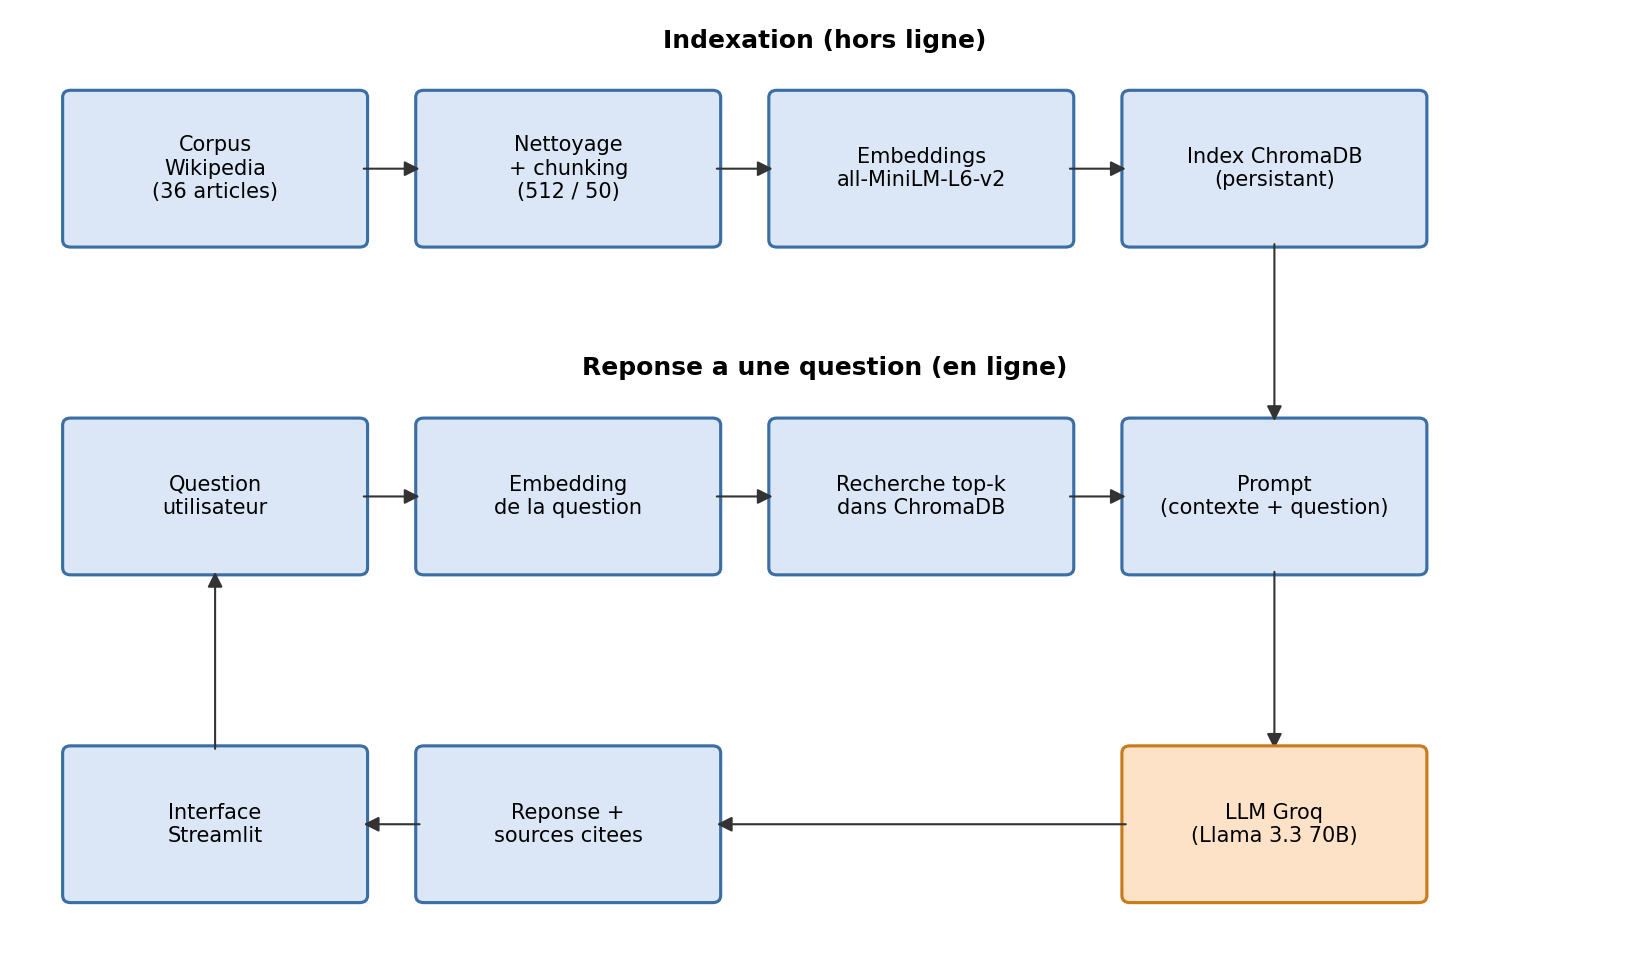
\includegraphics[width=\textwidth]{figures/architecture.png}
  \caption{Architecture g\'en\'erale du pipeline RAG (indexation hors ligne et r\'eponse en ligne).}
  \label{fig:archi}
\end{figure}

\subsection{Phase d'indexation (hors ligne)}

\begin{enumerate}[noitemsep]
  \item \textbf{Corpus} : 36 articles Wikipedia t\'el\'echarg\'es par \texttt{collect\_corpus.py}.
  \item \textbf{Nettoyage et chunking} : suppression des pages d'homonymie et des sections
        non informatives, puis d\'ecoupage en chunks de 512 caract\`eres avec un chevauchement
        de 50 caract\`eres (\texttt{src/prepare\_data.py}).
  \item \textbf{Embeddings} : chaque chunk est vectoris\'e avec \texttt{all-MiniLM-L6-v2}
        (\texttt{sentence-transformers}).
  \item \textbf{Index vectoriel} : vecteurs, textes et m\'etadonn\'ees (document source) stock\'es
        dans une collection ChromaDB persistante (\texttt{src/build\_index.py}).
\end{enumerate}

\subsection{Phase de r\'eponse (en ligne)}

\begin{enumerate}[noitemsep]
  \item La question utilisateur est encod\'ee avec le m\^eme mod\`ele d'embedding.
  \item ChromaDB renvoie les \texttt{top-3} chunks les plus proches (similarit\'e cosinus).
  \item Ces chunks sont ins\'er\'es dans un template de prompt avec la question.
  \item Le prompt est envoy\'e au LLM via l'API Groq (\texttt{llama-3.3-70b-versatile}).
  \item La r\'eponse et les sources sont affich\'ees dans le CLI ou l'interface Streamlit.
\end{enumerate}

\subsection{Organisation du d\'ep\^ot}

Le code source est versionn\'e sur GitHub :
\url{https://github.com/Muhammed-OTP/rag-nlp-m1}. Les param\`etres partag\'es (taille de chunk,
chevauchement, mod\`ele d'embedding, \texttt{top\_k}, mod\`ele Groq) sont centralis\'es dans
\texttt{config.py} pour \'eviter toute duplication.

\section{Donn\'ees et pr\'eparation du corpus}
\label{sec:donnees}

\subsection{Source et contenu}

Le corpus est constitu\'e de \textbf{36 articles Wikipedia en anglais}, couvrant les principaux
concepts du NLP et du machine learning abord\'es dans le module (mod\`eles de langage, embeddings,
architectures neuronales, m\'etriques d'\'evaluation, etc.). Les articles sont t\'el\'echarg\'es
automatiquement avec la biblioth\`eque \texttt{wikipedia} et sauvegard\'es en texte brut dans
\texttt{data/raw/}.

\subsection{Nettoyage}

Deux articles se sont r\'ev\'el\'es \`etre des pages d'homonymie (\emph{BM25} et
\emph{Tokenization}) sans contenu encyclop\'edique exploitable ; ils ont \'et\'e \'ecart\'es. Le
sujet de la tokenisation est d\'ej\`a couvert par l'article \emph{Tokenization (lexical analysis)}.
Le corpus final compte donc \textbf{34 documents}, ce qui respecte la contrainte minimale de
30 documents impos\'ee par le sujet.

Pour chaque document conserv\'e, les sections de fin g\'en\'eriques (\emph{See also},
\emph{References}, \emph{Notes}, \emph{External links}) sont supprim\'ees afin de ne garder que
le contenu pertinent.

\subsection{D\'ecoupage en chunks}

Chaque document nettoy\'e est d\'ecoup\'e en chunks de \textbf{512 caract\`eres} avec un
chevauchement de \textbf{50 caract\`eres} entre chunks cons\'ecutifs. Ce chevauchement limite le
risque qu'une information importante soit coup\'ee entre deux segments et perdue lors de la
recherche. Le d\'ecoupage produit \textbf{1443 chunks}, stock\'es au format JSON Lines dans
\texttt{data/processed/chunks.jsonl} (identifiant, document source, texte).

\subsection{Liste des documents}

Le tableau~\ref{tab:corpus} liste les 34 articles utilis\'es (titres originaux en anglais).

\begin{table}[H]
  \centering
  \caption{Articles Wikipedia du corpus (34 documents).}
  \label{tab:corpus}
  \small
  \begin{tabular}{@{}p{0.46\textwidth}p{0.46\textwidth}@{}}
    \toprule
    \textbf{Document} & \textbf{Document} \\
    \midrule
    Attention (machine learning) & BERT (language model) \\
    BLEU & Bag-of-words model \\
    Cosine similarity & FastText \\
    Fine-tuning (deep learning) & GPT (language model) \\
    GloVe (machine learning) & Hallucination (artificial intelligence) \\
    Information retrieval & LangChain \\
    Lemmatization & Long short-term memory \\
    N-gram & Named-entity recognition \\
    Perplexity (natural language processing) & Question answering (computing) \\
    ROUGE (metric) & Recurrent neural network \\
    Retrieval-augmented generation & Sentence embedding \\
    Sentiment analysis & Seq2seq \\
    Stemming & Stop word \\
    TF-IDF & Text classification \\
    Text segmentation & Tokenization (lexical analysis) \\
    Transfer learning & Transformer (machine learning) \\
    Vector database & Word2vec \\
    \bottomrule
  \end{tabular}
\end{table}

\section{Impl\'ementation}
\label{sec:impl}

\subsection{Choix techniques}

Les choix techniques sont r\'esum\'es dans le tableau~\ref{tab:tech}. Tous les param\`etres
num\'eriques proviennent de \texttt{config.py}.

\begin{table}[H]
  \centering
  \caption{Choix techniques et justifications.}
  \label{tab:tech}
  \small
  \begin{tabular}{@{}p{2.4cm}p{3.2cm}p{7.8cm}@{}}
    \toprule
    \textbf{Composant} & \textbf{Choix} & \textbf{Justification} \\
    \midrule
    Langage & Python 3.13 & \'Ecosyst\`eme NLP mature (sentence-transformers, ChromaDB, Streamlit). \\
    Embeddings & all-MiniLM-L6-v2 & Mod\`ele compact ($\sim$80~Mo), rapide en CPU, adapt\'e \`a la recherche s\'emantique. \\
    Base vectorielle & ChromaDB (persistant) & Int\'egration simple, pas de serveur externe, persistance locale. \\
    LLM & Groq --- llama-3.3-70b-versatile & API rapide, mod\`ele open-weight performant. \\
    Interface & Streamlit + CLI & CLI pour le d\'eveloppement ; Streamlit pour la d\'emo interactive. \\
    D\'ecoupage & 512 / overlap 50 & Compromis granularit\'e / contexte par chunk. \\
    Top-k & 3 & Suffisant pour couvrir la r\'eponse sans diluer le contexte. \\
    \bottomrule
  \end{tabular}
\end{table}

\subsection{Pipeline de r\'ecup\'eration et de g\'en\'eration}

Le module \texttt{src/rag\_pipeline.py} impl\'emente les fonctions centrales :
\begin{itemize}[noitemsep]
  \item \texttt{retrieve()} : encode la question et interroge ChromaDB ;
  \item \texttt{build\_prompt()} : assemble le contexte r\'ecup\'er\'e et la question ;
  \item \texttt{generate\_answer()} : appelle le LLM Groq et retourne la r\'eponse ainsi que
        les chunks sources.
\end{itemize}

Le template de prompt demande explicitement au mod\`ele de r\'epondre \textbf{uniquement} \`a partir
du contexte fourni et d'indiquer s'il ne conna\^it pas la r\'eponse, afin de limiter les
hallucinations. Un extrait est donn\'e en annexe~\ref{ann:code}.

\subsection{Interface utilisateur}

\subsubsection{Ligne de commande (op\'erationnelle)}

La commande \texttt{python -m src.rag\_pipeline} lance une boucle interactive : l'utilisateur
pose une question, le syst\`eme affiche la r\'eponse et les documents sources. Cette interface
a servi de base pour valider le pipeline avant l'\'evaluation automatique.

\subsubsection{Streamlit (impl\'ement\'ee, validation en cours)}

L'application \texttt{app.py} organise l'interface en trois onglets :
\begin{itemize}[noitemsep]
  \item \textbf{Chat} : conversation avec affichage du temps de r\'eponse, des chunks utilis\'es,
        d'un score de fid\'elit\'e et des extraits sources ;
  \item \textbf{\'Evaluation} : chargement d'un jeu de questions (JSON/CSV), lancement de
        l'\'evaluation, m\'etriques agr\'eg\'ees, graphiques Plotly et export CSV/PDF ;
  \item \textbf{Gestion du corpus} : statistiques, ajout de documents (PDF/TXT), s\'election des
        sources et reconstruction de l'index vectoriel.
\end{itemize}

La barre lat\'erale permet de choisir le mod\`ele LLM Groq, d'ajuster \texttt{top-k} et le seuil
de similarit\'e. Les tests finaux de cette interface et la pr\'eparation de la d\'emonstration
orale constituent le travail restant identifi\'e en section~\ref{sec:etat}.

\subsection{Scripts principaux}

\begin{table}[H]
  \centering
  \caption{Scripts du projet et r\^ole.}
  \label{tab:scripts}
  \small
  \begin{tabular}{@{}p{4.5cm}p{9cm}@{}}
    \toprule
    \textbf{Fichier} & \textbf{R\^ole} \\
    \midrule
    \texttt{collect\_corpus.py} & T\'el\'echargement des articles Wikipedia \\
    \texttt{src/prepare\_data.py} & Nettoyage et chunking \\
    \texttt{src/build\_index.py} & Embeddings et index ChromaDB \\
    \texttt{src/rag\_pipeline.py} & R\'ecup\'eration + g\'en\'eration (CLI) \\
    \texttt{app.py} & Interface Streamlit \\
    \texttt{evaluation/evaluate.py} & \'Evaluation batch sur le jeu de test \\
    \texttt{visualizations/plot\_results.py} & G\'en\'eration des graphiques \\
    \bottomrule
  \end{tabular}
\end{table}

\section{M\'ethodologie d'\'evaluation}
\label{sec:methode}

\subsection{Jeu de questions}

Un jeu de \textbf{34 questions} a \'et\'e constitu\'e manuellement
(\texttt{evaluation/eval\_questions.json}), couvrant l'ensemble des 34 documents du corpus ---
une question par concept, plus quelques questions \`a sources multiples lorsque les notions sont
\'etroitement li\'ees (par exemple lemmatisation / stemmatisation, ou LSTM / RNN). Ce jeu d\'epasse
le minimum de 20 questions exig\'e par le sujet du projet.

Chaque entr\'ee contient :
\begin{itemize}[noitemsep]
  \item la \textbf{question} en anglais (langue du corpus) ;
  \item la liste des \textbf{documents attendus} (\texttt{expected\_sources}).
\end{itemize}

\subsection{M\'etriques calcul\'ees}

Pour chaque question, le script \texttt{evaluation/evaluate.py} ex\'ecute le pipeline complet
(r\'ecup\'eration + g\'en\'eration) et calcule quatre m\'etriques :

\begin{description}
  \item[Precision@3] Proportion des 3 chunks r\'ecup\'er\'es qui appartiennent au(x) document(s)
        attendu(s). Mesure la pr\'ecision du retriever.
  \item[Recall@3] Proportion des documents attendus pr\'esents parmi les chunks r\'ecup\'er\'es.
        Indique si l'information n\'ecessaire a \'et\'e retrouv\'ee.
  \item[Fid\'elit\'e (faithfulness)] Proportion des mots de la r\'eponse g\'en\'er\'ee qui
        apparaissent \'egalement dans le contexte r\'ecup\'er\'e --- mesure lexicale simple de
        l'ancrage de la r\'eponse dans les sources (proxy de l'absence d'hallucination).
  \item[Temps de r\'eponse] Dur\'ee totale (secondes) incluant l'encodage de la question, la
        recherche vectorielle et l'appel \`a l'API Groq.
\end{description}

Les r\'esultats d\'etaill\'es (une ligne par question) sont sauvegard\'es dans
\texttt{evaluation/results.csv}. Les graphiques de la section~\ref{sec:resultats} sont produits
par \texttt{visualizations/plot\_results.py} \`a partir de ce fichier.

\subsection{Reproductibilit\'e}

Pour reproduire l'\'evaluation :
\begin{enumerate}[noitemsep]
  \item Construire l'index : \texttt{python -m src.build\_index}
  \item Configurer \texttt{GROQ\_API\_KEY} dans un fichier \texttt{.env}
  \item Lancer : \texttt{python -m evaluation.evaluate}
  \item G\'en\'erer les figures : \texttt{python -m visualizations.plot\_results}
\end{enumerate}

Les r\'esultats pr\'esent\'es dans ce rapport proviennent d'une ex\'ecution compl\`ete de cette
cha\^ine sur la machine de d\'eveloppement (juin 2026).

\section{R\'esultats et visualisations}
\label{sec:resultats}

L'\'evaluation a \'et\'e ex\'ecut\'ee sur les 34 questions du jeu de test. Le
tableau~\ref{tab:metrics} r\'esume les moyennes obtenues.

\begin{table}[H]
  \centering
  \caption{Moyennes des m\'etriques d'\'evaluation (34 questions).}
  \label{tab:metrics}
  \begin{tabular}{@{}lc@{}}
    \toprule
    \textbf{M\'etrique} & \textbf{Valeur moyenne} \\
    \midrule
    Precision@3 & 0.922 \\
    Recall@3 & 0.985 \\
    Fid\'elit\'e (faithfulness) & 0.887 \\
    Temps de r\'eponse (s) & 0.811 \\
    \bottomrule
  \end{tabular}
\end{table}

\subsection{Synth\`ese des m\'etriques}

La figure~\ref{fig:avg} pr\'esente les moyennes des trois scores principaux (precision, recall,
fid\'elit\'e). Le recall moyen tr\`es \'elev\'e (0.985) indique que le retriever retrouve
quasi syst\'ematiquement au moins un chunk du document attendu. La precision l\'eg\`erement
inf\'erieure (0.922) refl\`ete des cas o\`u un ou deux des trois chunks proviennent de documents
voisins s\'emantiquement proches (voir section~\ref{sec:discussion}).

\begin{figure}[H]
  \centering
  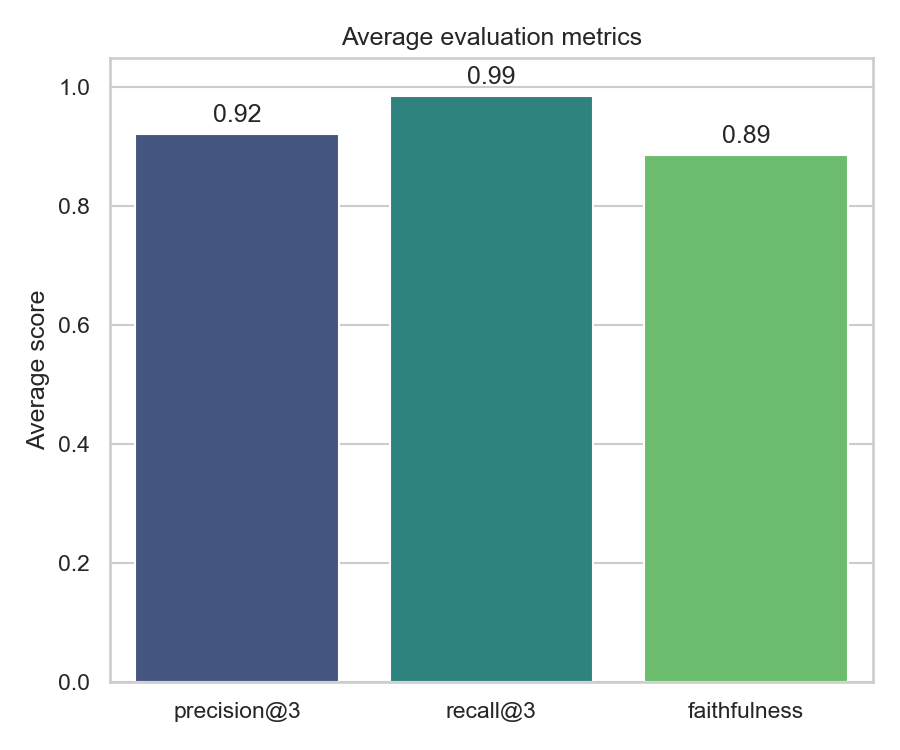
\includegraphics[width=0.62\textwidth]{figures/average_metrics.png}
  \caption{Moyennes des m\'etriques d'\'evaluation sur les 34 questions.}
  \label{fig:avg}
\end{figure}

\subsection{Precision et recall par question}

La figure~\ref{fig:pr} d\'etaille Precision@3 et Recall@3 pour chaque question. La majorit\'e
des questions atteignent un score de 1.0 ; quelques exceptions correspondent \`a des sujets
proches (FastText / Word2vec, lemmatisation / stemmatisation, etc.).

\begin{figure}[H]
  \centering
  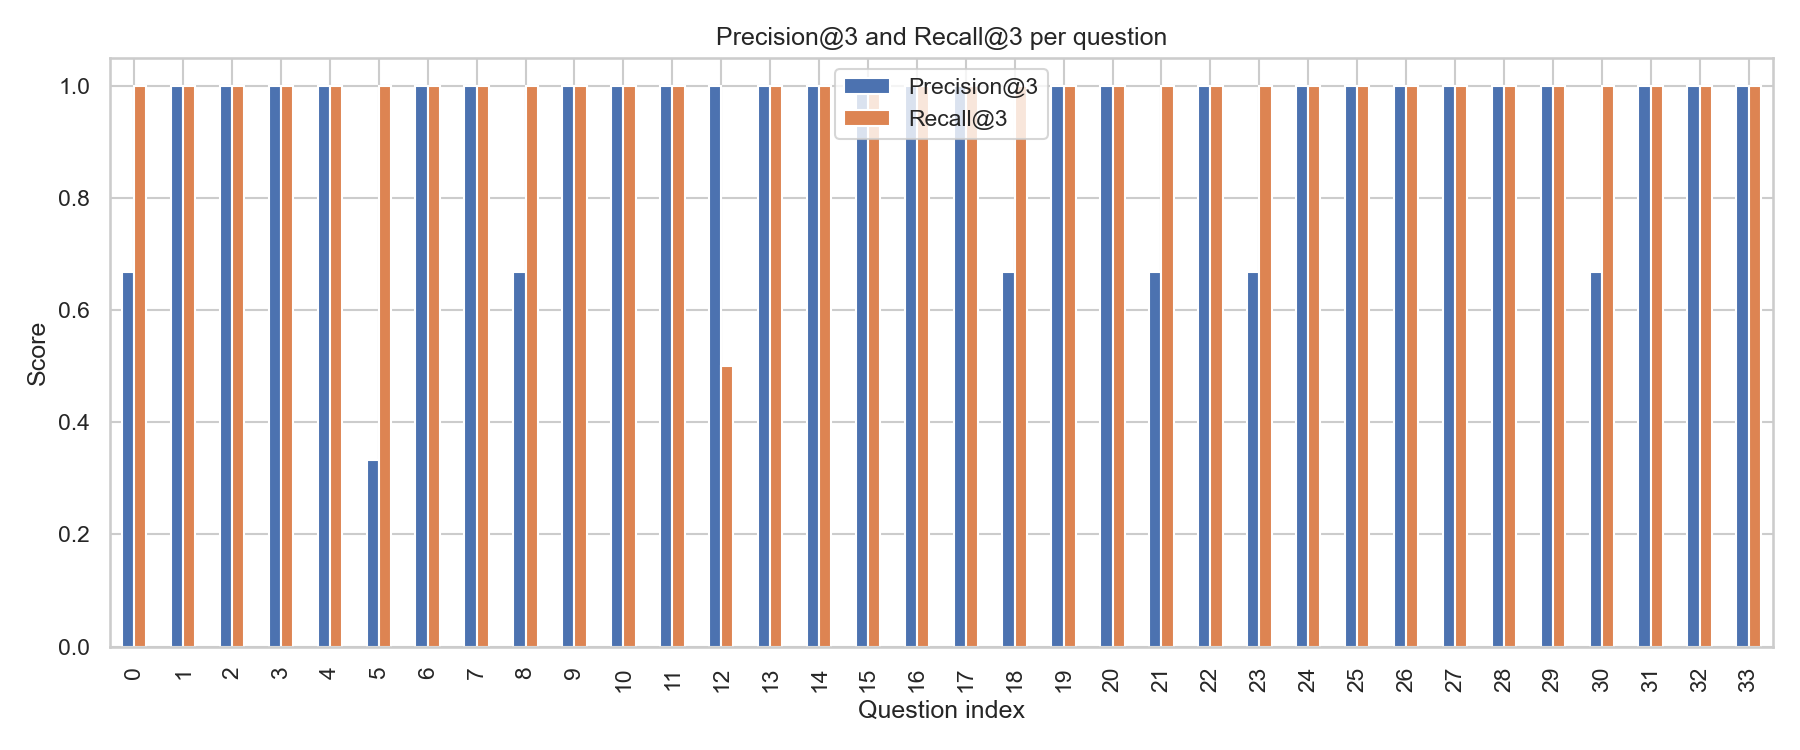
\includegraphics[width=\textwidth]{figures/precision_recall_per_question.png}
  \caption{Precision@3 et Recall@3 pour chacune des 34 questions.}
  \label{fig:pr}
\end{figure}

\subsection{Distribution de la fid\'elit\'e}

La figure~\ref{fig:faith} montre la distribution du score de fid\'elit\'e lexicale. La plupart
des r\'eponses d\'epassent 0.8, ce qui indique un bon ancrage dans le contexte r\'ecup\'er\'e.
Quelques scores plus bas (par exemple pour la question sur BERT, fid\'elit\'e = 0.484) s'expliquent
par des reformulations correctes utilisant un vocabulaire diff\'erent de celui des chunks, limite
connue de la m\'etrique lexicale.

\begin{figure}[H]
  \centering
  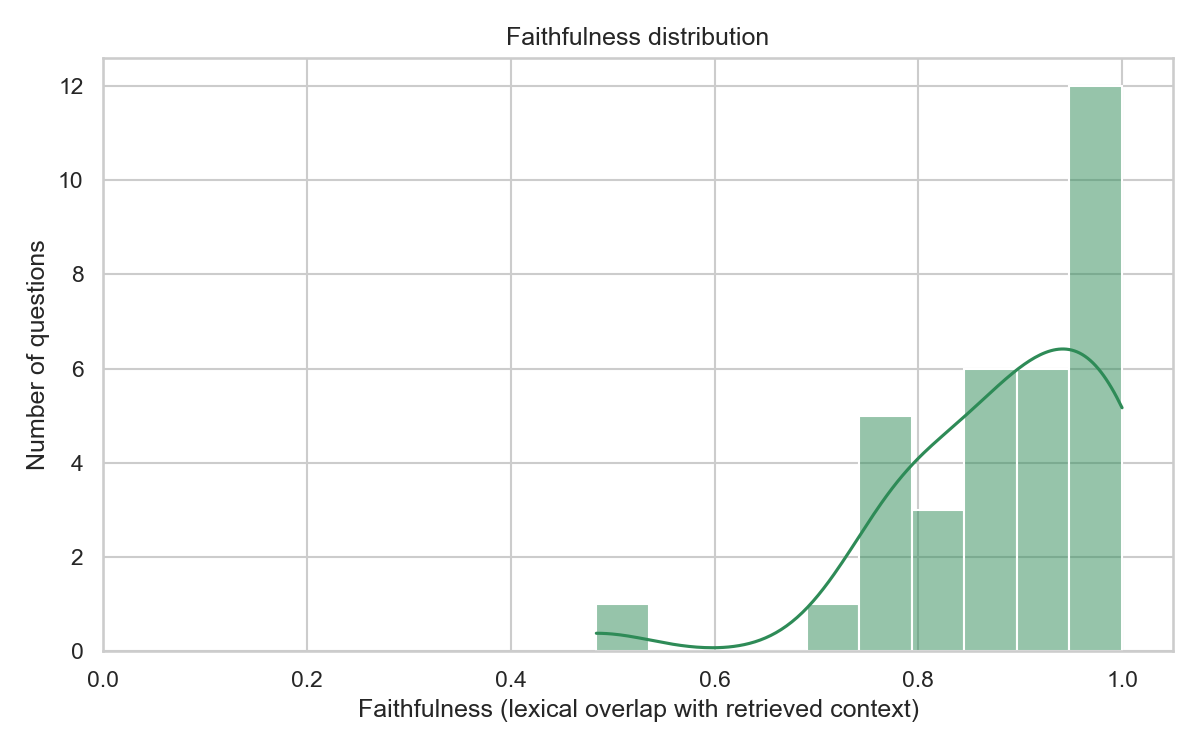
\includegraphics[width=0.72\textwidth]{figures/faithfulness_distribution.png}
  \caption{Distribution du score de fid\'elit\'e (recouvrement lexical avec le contexte).}
  \label{fig:faith}
\end{figure}

\subsection{Temps de r\'eponse}

La figure~\ref{fig:time} pr\'esente la distribution des temps de r\'eponse. La majorit\'e des
questions sont trait\'ees en moins d'une seconde ; quelques valeurs plus \'elev\'ees (jusqu'\`a
3.5~s) correspondent \`a des r\'eponses plus longues ou \`a une latence r\'eseau ponctuelle de
l'API Groq.

\begin{figure}[H]
  \centering
  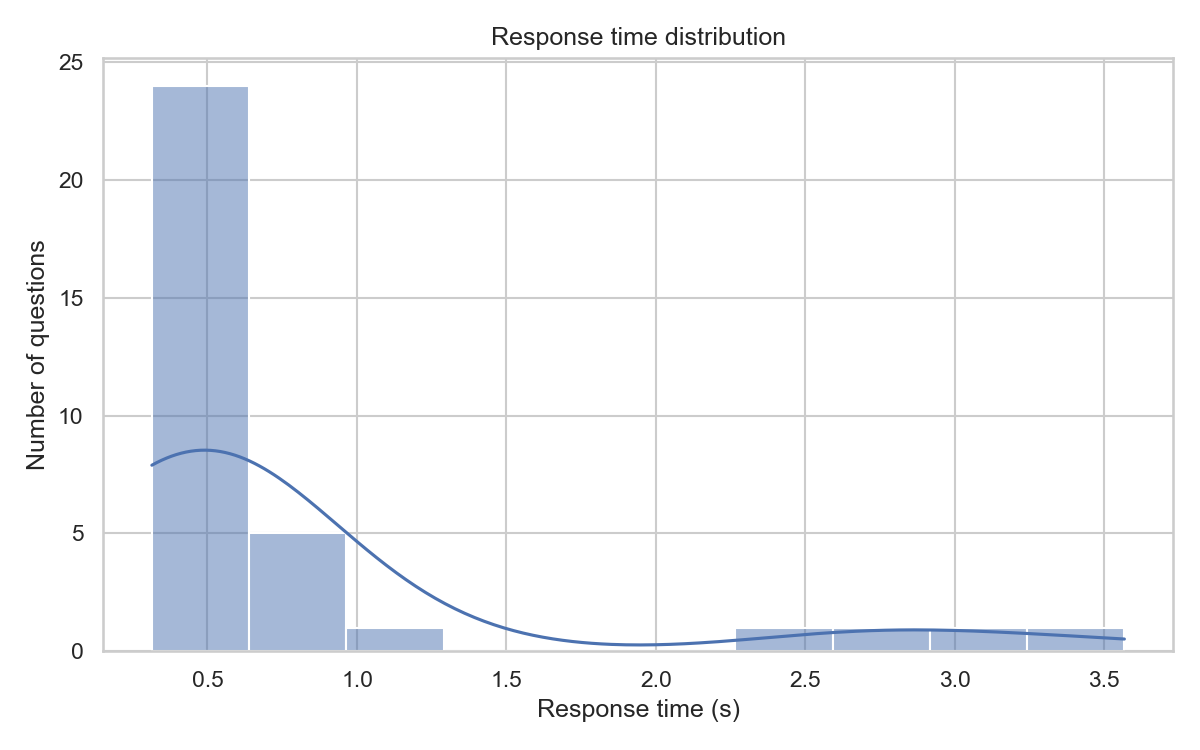
\includegraphics[width=0.72\textwidth]{figures/response_time_distribution.png}
  \caption{Distribution des temps de r\'eponse (secondes).}
  \label{fig:time}
\end{figure}

\subsection{Relation temps / fid\'elit\'e}

La figure~\ref{fig:scatter} croise temps de r\'eponse, fid\'elit\'e et precision@3. Aucune
corr\'elation forte n'appara\^it : une r\'eponse plus lente n'est ni syst\'ematiquement plus
fid\`ele, ni moins pr\'ecise.

\begin{figure}[H]
  \centering
  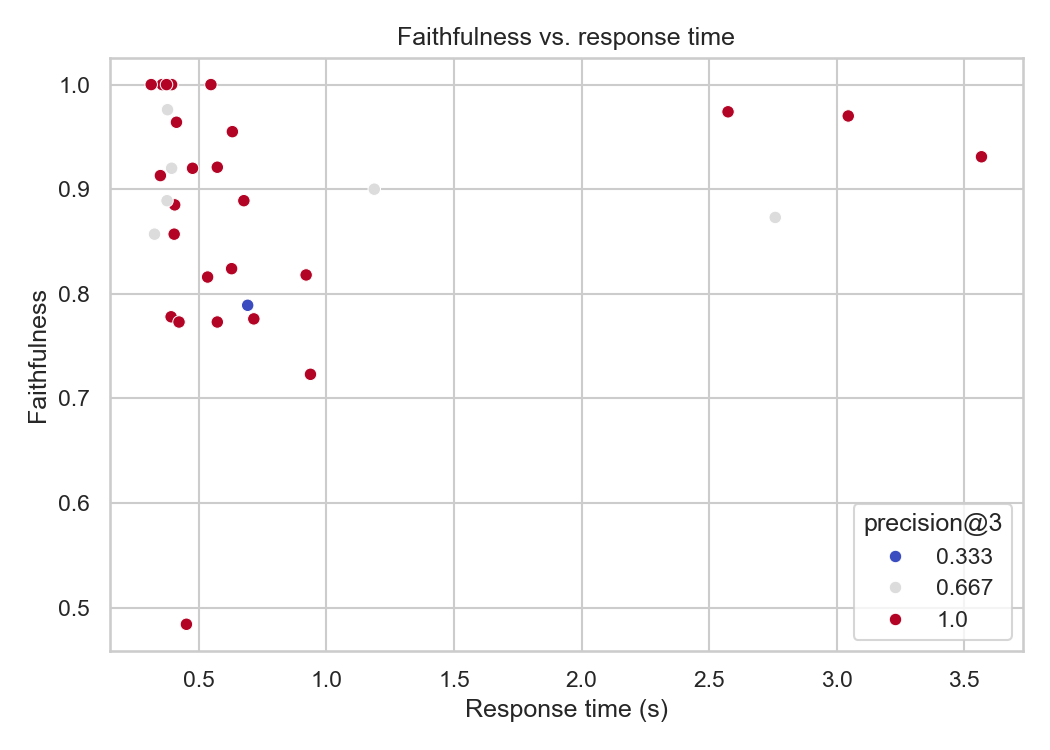
\includegraphics[width=0.72\textwidth]{figures/time_vs_faithfulness.png}
  \caption{Temps de r\'eponse, fid\'elit\'e et precision@3 (couleur).}
  \label{fig:scatter}
\end{figure}

\subsection{Questions \`a scores plus faibles (extrait)}

\begin{table}[H]
  \centering
  \caption{Exemples de questions avec precision@3 inf\'erieure \`a 1.0.}
  \label{tab:lowprec}
  \small
  \begin{tabular}{@{}p{5.8cm}cc@{}}
    \toprule
    \textbf{Question (abr\'eg\'ee)} & \textbf{Prec.@3} & \textbf{Recall@3} \\
    \midrule
    FastText vs earlier embeddings & 0.333 & 1.0 \\
    Attention mechanism in ML & 0.667 & 1.0 \\
    GloVe word vectors training & 0.667 & 1.0 \\
    Lemmatization vs stemming & 1.0 & 0.5 \\
    Sentence embedding uses & 0.667 & 1.0 \\
    \bottomrule
  \end{tabular}
\end{table}

Ces cas illustrent la difficult\'e d'attribuer un unique document ``gold'' lorsque plusieurs
articles du corpus traitent de notions voisines.

\section{Discussion}
\label{sec:discussion}

\subsection{Points forts}

\begin{itemize}
  \item Le pipeline principal (collecte, indexation, RAG CLI) est \textbf{fonctionnel de bout en
        bout} et produit des r\'eponses ancr\'ees dans les sources Wikipedia du domaine NLP/ML.
  \item Les r\'esultats d'\'evaluation montrent un \textbf{recall@3 moyen de 0.985} et une
        \textbf{precision@3 moyenne de 0.922} : le retriever bas\'e sur \texttt{all-MiniLM-L6-v2}
        retrouve quasi syst\'ematiquement le bon document, m\^eme pour des formulations diff\'erentes
        du texte source.
  \item La \textbf{fid\'elit\'e moyenne de 0.887} et le prompt restrictif limitent les
        hallucinations dans la majorit\'e des cas observ\'es.
  \item Le \textbf{temps de r\'eponse moyen de 0.81~s} rend le syst\`eme utilisable de mani\`ere
        interactive via le CLI (et, une fois valid\'ee, via Streamlit).
  \item Le d\'ep\^ot GitHub documente chaque phase (\texttt{PHASES.md}) et centralise les
        param\`etres dans \texttt{config.py}, ce qui facilite la reproductibilit\'e.
\end{itemize}

\subsection{Limites et travail en cours}

\begin{itemize}
  \item \textbf{Documents voisins} : pour des sujets proches (FastText / Word2vec, sentence
        embedding / BERT), le retriever renvoie parfois des chunks pertinents s\'emantiquement mais
        issus d'un document diff\'erent de celui marqu\'e comme ``attendu'', ce qui p\'enalise la
        precision@3 sans invalider la qualit\'e de la r\'eponse.
  \item \textbf{M\'etrique de fid\'elit\'e lexicale} : elle ne d\'etecte ni les reformulations
        correctes (synonymes) ni les hallucinations subtiles r\'eutilisant le vocabulaire du
        contexte. Une \'evaluation par LLM-as-judge serait plus fine mais plus co\^uteuse.
  \item \textbf{Corpus en anglais} : le syst\`eme r\'epond en anglais et ne couvre que le contenu
        des articles t\'el\'echarg\'es ; il ne refl\`ete pas les avanc\'ees post\'erieures au
        t\'el\'echargement.
  \item \textbf{Interface Streamlit} : impl\'ement\'ee avec des fonctionnalit\'es avanc\'es
        (\'evaluation int\'egr\'ee, gestion du corpus), mais sa validation utilisateur finale et
        la pr\'eparation de la d\'emonstration orale restent en cours au moment de la r\'edaction.
  \item \textbf{Pas de re-ranking} : la recherche vectorielle seule ne desambiguise pas les
        articles tr\`es proches ; un cross-encoder ou un filtrage par m\'etadonn\'ees pourrait
        am\'eliorer la precision.
\end{itemize}

\subsection{Alignement avec le sujet du projet}

Le projet respecte les exigences principales du sujet : corpus $\geq$30 documents, index
vectoriel, pipeline RAG avec LLM, interface (CLI + Streamlit), jeu de test $\geq$20 questions,
m\'etriques demand\'ees et graphiques de performance. Les parties encore en cours (tests Streamlit,
README final, d\'emo) sont explicitement signal\'ees et n'invalident pas les r\'esultats
d'\'evaluation obtenus sur le pipeline principal.

\section{Conclusion et perspectives}
\label{sec:conclusion}

Ce projet a permis de mettre en \oe uvre l'essentiel de la cha\^ine d'un syst\`eme RAG appliqu\'e
aux concepts NLP/ML : constitution d'un corpus Wikipedia, pr\'eparation des donn\'ees, indexation
vectorielle avec ChromaDB, pipeline de r\'ecup\'eration et de g\'en\'eration via Groq, \'evaluation
quantitative sur 34 questions et visualisation des performances.

Les r\'esultats obtenus (precision@3 = 0.922, recall@3 = 0.985, fid\'elit\'e = 0.887, temps
moyen = 0.811~s) montrent que le syst\`eme r\'epond de mani\`ere pertinente et rapide sur
l'ensemble du corpus choisi. L'interface Streamlit a \'et\'e valid\'ee par des tests interactifs confirmant la qualit\'e
des r\'eponses en conditions d'utilisation r\'eelle. La documentation (\texttt{README.md}) et
le script de d\'emonstration (\texttt{DEMO.md}) accompagnent la soutenance du 15 juin 2026.

\subsection{Perspectives}

\begin{itemize}[noitemsep]
  \item Remplacer la m\'etrique de fid\'elit\'e lexicale par une approche LLM-as-judge.
  \item Ajouter un re-ranking (cross-encoder) pour am\'eliorer la precision sur les sujets
        recouvrants.
  \item \'Etendre le corpus (sources r\'ecentes, contenu multilingue).
  \item Permettre la citation explicite des sources dans le texte de la r\'eponse g\'en\'er\'ee.
\end{itemize}

Le code source, les scripts d'\'evaluation et ce rapport LaTeX sont disponibles sur le d\'ep\^ot :
\url{https://github.com/Muhammed-OTP/rag-nlp-m1}.

\section{R\'ef\'erences}
\label{sec:refs}

\begin{itemize}[leftmargin=*]
  \item Wikipedia, articles divers sur les concepts de NLP et de machine learning
        (\url{https://en.wikipedia.org}), consult\'es en juin 2026.
  \item Reimers, N. \& Gurevych, I. (2019). \emph{Sentence-BERT: Sentence Embeddings using Siamese
        BERT-Networks}. EMNLP. (mod\`ele \texttt{all-MiniLM-L6-v2})
  \item Vaswani, A. et al. (2017). \emph{Attention Is All You Need}. NeurIPS.
  \item Lewis, P. et al. (2020). \emph{Retrieval-Augmented Generation for Knowledge-Intensive NLP
        Tasks}. NeurIPS.
  \item Documentation ChromaDB --- \url{https://docs.trychroma.com/}
  \item Documentation Groq API --- \url{https://console.groq.com/docs/}
  \item Documentation Streamlit --- \url{https://docs.streamlit.io/}
  \item Documentation sentence-transformers --- \url{https://www.sbert.net/}
  \item Sujet du projet RAG, Module NLP M1 --- \texttt{Sujet\_Projet\_RAG.pdf}
  \item D\'ep\^ot GitHub du projet --- \url{https://github.com/Muhammed-OTP/rag-nlp-m1}
\end{itemize}


\appendix
\section{Extraits de code}
\label{ann:code}

\subsection{Template de prompt (\texttt{src/rag\_pipeline.py})}

\begin{lstlisting}[style=python,caption={Template de prompt limitant les hallucinations.}]
PROMPT_TEMPLATE = """Answer the question using only the context below. \
If the context does not contain the answer, say you don't know.

Context:
{context}

Question: {question}

Answer:"""
\end{lstlisting}

\subsection{Fonction de r\'ecup\'eration}

\begin{lstlisting}[style=python,caption={R\'ecup\'eration des top-k chunks depuis ChromaDB.}]
def retrieve(question, model, collection, top_k=TOP_K):
    query_embedding = model.encode([question])
    results = collection.query(
        query_embeddings=query_embedding.tolist(),
        n_results=top_k,
    )
    chunks = []
    for chunk_id, text, meta in zip(
        results["ids"][0],
        results["documents"][0],
        results["metadatas"][0],
    ):
        chunks.append({
            "id": chunk_id,
            "text": text,
            "source": meta["source"],
        })
    return chunks
\end{lstlisting}

\subsection{Calcul de la fid\'elit\'e (\texttt{evaluation/evaluate.py})}

\begin{lstlisting}[style=python,caption={Recouvrement lexical entre reponse et contexte.}]
def lexical_overlap(answer: str, context: str) -> float:
    answer_tokens = set(re.findall(r"\w+", answer.lower()))
    context_tokens = set(re.findall(r"\w+", context.lower()))
    if not answer_tokens:
        return 0.0
    return len(answer_tokens & context_tokens) / len(answer_tokens)
\end{lstlisting}

\subsection{Param\`etres partag\'es (\texttt{config.py})}

\begin{lstlisting}[style=python,caption={Constantes centralisees du projet.}]
CHUNK_SIZE = 512
CHUNK_OVERLAP = 50
EMBEDDING_MODEL = "all-MiniLM-L6-v2"
TOP_K = 3
GROQ_MODEL = "llama-3.3-70b-versatile"
\end{lstlisting}

\section{Exemples question-r\'eponse}
\label{ann:exemples}

Les exemples suivants proviennent de l'ex\'ecution du pipeline sur le jeu d'\'evaluation
(\texttt{evaluation/results.csv}). Ils illustrent un cas \`a haute performance et un cas o\`u la
precision@3 est p\'enalis\'ee par la proximit\'e s\'emantique entre documents voisins.

\subsection{Exemple 1 --- Performance \'elev\'ee}

\textbf{Question :} \emph{What is retrieval-augmented generation and what problem does it address?}

\textbf{Sources attendues :} Retrieval-augmented generation

\textbf{Sources r\'ecup\'er\'ees :} Retrieval-augmented generation (x3)

\textbf{M\'etriques :} Precision@3 = 1.0, Recall@3 = 1.0, Fid\'elit\'e = 0.776, Temps = 0.716~s

\textbf{Interpr\'etation :} les trois chunks proviennent du bon article ; le retriever et le LLM
produisent une r\'eponse directement ancr\'ee dans la d\'efinition Wikipedia du RAG.

\subsection{Exemple 2 --- Documents voisins}

\textbf{Question :} \emph{What is FastText and how does it differ from earlier word embedding methods?}

\textbf{Sources attendues :} FastText

\textbf{Sources r\'ecup\'er\'ees :} FastText; Word2vec; BERT (language model)

\textbf{M\'etriques :} Precision@3 = 0.333, Recall@3 = 1.0, Fid\'elit\'e = 0.789, Temps = 0.692~s

\textbf{Interpr\'etation :} le chunk principal est correct (FastText), mais les deux suivants
proviennent d'articles li\'es aux embeddings (Word2vec, BERT). La r\'eponse reste pertinente pour
l'utilisateur, mais la m\'etrique precision@3 est p\'enalis\'ee car seul un chunk sur trois
correspond au document ``gold'' d\'efini manuellement.

\subsection{Exemple 3 --- Recall partiel (sources multiples)}

\textbf{Question :} \emph{What is lemmatization and how does it differ from stemming?}

\textbf{Sources attendues :} Lemmatization; Stemming

\textbf{Sources r\'ecup\'er\'ees :} Lemmatization (x3)

\textbf{M\'etriques :} Precision@3 = 1.0, Recall@3 = 0.5, Fid\'elit\'e = 0.824, Temps = 0.629~s

\textbf{Interpr\'etation :} tous les chunks proviennent de l'article sur la lemmatisation, mais
l'article sur le \emph{stemming} n'appara\^it pas dans le top-3 ; le recall@3 est donc de 0.5
alors que la r\'eponse peut n\'eanmoins mentionner les deux notions via le contenu du chunk
r\'ecup\'er\'e.

\subsection{Lancement du CLI}

\begin{lstlisting}[style=python,caption={Commande pour interroger le systeme en ligne de commande.}]
# Apres construction de l'index et configuration de .env
python -m src.rag_pipeline

# Exemple de question interactive :
# > What is the transformer architecture and why was it introduced?
\end{lstlisting}

\begin{lstlisting}[style=python,caption={Lancement de l'interface Streamlit.}]
streamlit run app.py
\end{lstlisting}


\end{document}
